\documentclass{sigplanconf}

\usepackage{ifthen}
\usepackage{fancyvrb}
\usepackage{color}
\usepackage{ulem}
\usepackage{xspace}
\usepackage{epsfig}
\usepackage{amssymb}
\usepackage{amsmath}
\usepackage{amsfonts}
\usepackage[utf8]{inputenc}

\newboolean{showcomments}
\setboolean{showcomments}{false}
\ifthenelse{\boolean{showcomments}}
  {\newcommand{\nb}[2]{
    \fbox{\bfseries\sffamily\scriptsize#1}
    {\sf\small$\blacktriangleright$\textit{#2}$\blacktriangleleft$}
   }
   \newcommand{\version}{\emph{\scriptsize$-$Id: main.tex 19055 2008-06-05 11:20:31Z cfbolz $-$}}
  }
  {\newcommand{\nb}[2]{}
   \newcommand{\version}{}
  }

\newcommand\cfbolz[1]{\nb{CFB}{#1}}
\newcommand\arigo[1]{\nb{AR}{#1}}
\newcommand\fijal[1]{\nb{FIJAL}{#1}}
\newcommand\david[1]{\nb{DAVID}{#1}}
\newcommand\reva[1]{\nb{Reviewer 1}{#1}}
\newcommand\revb[1]{\nb{Reviewer 2}{#1}}
\newcommand\revc[1]{\nb{Reviewer 3}{#1}}
\newcommand{\commentout}[1]{}

\newcommand\ie{i.e.,\xspace}
\newcommand\eg{e.g.,\xspace}

\normalem

\let\oldcite=\cite

\renewcommand\cite[1]{\ifthenelse{\equal{#1}{XXX}}{[citation~needed]}{\oldcite{#1}}}

%
\def\sharedaffiliation{%
\end{tabular}
\begin{tabular}{c}}
%
\begin{document}
\conferenceinfo{PEPM'11,} {XXX}
\CopyrightYear{XXX}
\copyrightdata{XXX}

\title{Escape Analysis and Specialization in a Tracing JIT}

\authorinfo{Carl Friedrich Bolz \and Antonio Cuni \and Maciej Fijałkowski \and Samuele Pedroni \and Armin Rigo}
           {Heinrich-Heine-Universität Düsseldorf, STUPS Group, Germany XXX}
           {cfbolz@gmx.de XXX}

%\numberofauthors{3}
%\author{
%\alignauthor Carl Friedrich Bolz\\
%       \email{cfbolz@gmx.de}
%\alignauthor Michael Leuschel\\
%       \email{leuschel@cs.uni-duesseldorf.de}
%\alignauthor David Schneider\\
%      \email{david.schneider@uni-duesseldorf.de}
%      \sharedaffiliation
%      \affaddr{Heinrich-Heine-Universität Düsseldorf, STUPS Group, Germany}\\
%}

\maketitle
\begin{abstract}
\footnote{This research is partially supported by the BMBF funded project PyJIT (nr. 01QE0913B;
Eureka Eurostars).}
\end{abstract}

% A category with the (minimum) three required fields
%\category{H.4}{Information Systems Applications}{Miscellaneous}
%A category including the fourth, optional field follows...
%\category{D.2.8}{Software Engineering}{Metrics}[complexity measures, performance measures]

\category{D.3.4}{Programming Languages}{Processors}[code generation,
interpreters, run-time environments]

\terms
Languages, Performance, Experimentation

\keywords{XXX}%

XXX drop the word "allocation removal" somewhere

XXX define "escape analysis"

\section{Introduction}

XXX need to re-target introduction a bit to fit PEPMs focus

The goal of a just-in-time compiler for a dynamic language is obviously to
improve the speed of the language over an implementation of the language that
uses interpretation. The first goal of a JIT is thus to remove the
interpretation overhead, i.e. the overhead of bytecode (or AST) dispatch and the
overhead of the interpreter's data structures, such as operand stack etc. The
second important problem that any JIT for a dynamic language needs to solve is
how to deal with the overhead of boxing of primitive types and of type
dispatching. Those are problems that are usually not present or at least less
severe in statically typed languages.

Boxing of primitive types means that dynamic languages need to be able to handle
all objects, even integers, floats, bools etc. in the same way as user-defined
instances. Thus those primitive types are usually \emph{boxed}, i.e. a small
heap-structure is allocated for them, that contains the actual value. Boxing
primitive types can be very costly, because a lot of common operations,
particularly all arithmetic operations, have to produce a new box, in addition
to the actual computation they do. Because the boxes are allocated on the heap,
producing a lot of them puts pressure on the garbage collector.

Type dispatching is the process of finding the concrete implementation that is
applicable to the objects at hand when doing a generic operation on them. An
example would be the addition of two objects: The addition needs to check what
the concrete objects that should be added are, and choose the implementation
that is fitting for them. Type dispatching is a very common operation in a
dynamic language because no types are known at compile time, so all operations
need it.

A recently popular approach to implementing just-in-time compilers for dynamic
languages is that of a tracing JIT. A tracing JIT often takes the form of an
extension to an existing interpreter, which can be sped up that way. This
approach is also the one taken by the PyPy project, which is an environment for
implementing dynamic programming languages. PyPy's
approach to doing so is to straightforwardly implement an interpreter for the
to-be-implemented language, and then use powerful tools to turn the interpreter
into an efficient VM that also contains a just-in-time compiler. This compiler
is automatically generated from the interpreter using partial-evaluation-like
techniques \cite{bolz_tracing_2009}. The PyPy project and its approach to
tracing JIT compilers is described in Section~\ref{sec:Background}.

The tracing JIT approach that the PyPy project is taking removes the overhead
of bytecode dispatch. In this paper we want to explain how the traces that are
produced by PyPy's tracing JIT can be optimized to also remove some of the
overhead more closely associated to dynamic languages, such as boxing overhead
and type dispatching. To understand the problem more closely, we analyze the
occurring object lifetimes in Section~\ref{sec:lifetimes}. The most important
technique to achieve this is a form of escape analysis \cite{XXX} that we call
\emph{virtual objects},\footnote{The terminology comes from \cite{Psyco}}
which is described in Section~\ref{sec:virtuals}. The
goal of virtual objects is to remove allocations of temporary objects that have
a predictable lifetime and to optimize type dispatching in the process.

The basic approach of virtual objects can then be extended to also be used for
type-specializing the traces that are produced by the tracing JIT
(Section~\ref{sec:crossloop}). In Section~\ref{sec:XXX} we describe some
supporting techniques that are not central to the approach, but are needed to
improve the results. The introduced techniques are evaluated in
Section~\ref{sec:Evaluation} using PyPy's Python interpreter as a case study.

The contributions of this paper are:

\begin{enumerate}
    \item An efficient and effective algorithm for removing object allocations in a tracing JIT.
    \item XXX
\end{enumerate}

\section{Background}
\label{sec:Background}

\subsection{PyPy}
\label{sub:PyPy}

The work described in this paper was done in the context of the PyPy project
\cite{armin_rigo_pypys_2006}. PyPy is an environment where dynamic languages can
be implemented in a simple yet efficient way. The approach taken when
implementing a language with PyPy is to write an interpreter for the language in
\emph{RPython} \cite{davide_ancona_rpython:_2007}. RPython ("restricted Python")
is a subset of Python chosen in such a way, that type inference becomes
possible. The language interpreter can thus be translated with the help of
PyPy's tools into a VM on the C level. Because the interpreter is written at a
relatively high level, the language implementation is kept free of low-level
details, such as object layout, garbage collection or memory model. Those
aspects of the final VM are woven into the generated code during the translation
to C. XXX languages that are done using PyPy

The feature that makes PyPy more than a compiler with a runtime system is it's
support for automated JIT compiler generation \cite{bolz_tracing_2009}. During
the translation to C, PyPy's tools can generate a just-in-time compiler for the
language that the interpreter is implementing. This process is not fully
automatic, but needs to be guided by the language implementer by some
source-code hints. Semi-automatically generating a JIT compiler has many advantages
over writing one manually, which is an error-prone and tedious process. The
generated JIT has the same semantics as the interpreter by construction, and all
languages implemented using PyPy benefit from improvements to the JIT generator.
The JIT that is produced by PyPy's JIT generator is a \emph{tracing JIT
compiler}, a concept which will be explained in more detail in the next section.

\subsection{Tracing JIT Compilers}
\label{sub:JIT_background}

Tracing JITs are a recently more popular approach to write just-in-time
compilers for dynamic languages \cite{XXX}. Their origins lie in the Dynamo
project, that used a tracing approach to optimize machine code using execution
traces \cite{XXX}. They were then adapted to be used for a very light-weight
Java VM \cite{XXX} and afterwards used in several implementations of dynamic
languages, such as JavaScript \cite{XXX}, Lua \cite{XXX} and now Python via
PyPy.

The core idea of tracing JITs is to focus the optimization effort of the JIT
compiler on the hot paths of the core loops of the program and to just use an
interpreter for the less commonly executed parts. VMs that use a tracing JIT are
thus mixed-mode execution environments, they contain both an interpreter and a
JIT compiler. By default the interpreter is used to execute the program, doing
some light-weight profiling at the same time. This profiling is used to identify
the hot loops of the program. If a hot loop is found in that way, the
interpreter enters a special \emph{tracing mode}. In this tracing mode, the
interpreter records all operations that it is executing while running one
iteration of the hot loop. This history of executed operations of one loop is
called a \emph{trace}. Because the trace corresponds to one iteration of a loop,
it always ends with a jump to its own beginning.

This trace of operations is then the basis of the generated code. The trace is
optimized in some ways, and then turned into machine code. Generating machine
code is simple, because the traces are linear and the operations are very close
to machine level. The trace corresponds to one concrete execution of a loop,
therefore the code generated from it is only one possible path through the loop.
To make sure that the trace is maintaining the correct semantics, it contains a
\emph{guard} at all places where the execution could have diverged from the
path. Those guards check the assumptions under which execution can stay on the
trace. As an example, if a loop contains an \texttt{if} statement, the trace
will contain the execution of one of the paths only, which is the path that was
taken during the production of the trace. The trace will also contain a guard
that checks that the condition of the \texttt{if} statement is true, because if
it isn't, the rest of the trace is not valid.

When generating machine code, every guard is be turned into a quick check to
see whether the assumption still holds. When such a guard is hit during the
execution of the machine code and the assumption does not hold, the execution of
the machine code is stopped, and interpreter continues to run from that point
on. These guards are the only mechanism to stop the execution of a trace, the
loop end condition also takes the form of a guard.

bridges?

arguments to traces

getting from the interpreter to traces

XXX object model and its reflection in traces (e.g. guard\_class before each method call)

\subsection{Running Example}

For the purpose of this paper, we are going to use a very simple object
model, that just supports an integer and a float type. The objects support only
two operations, \texttt{add}, which adds two objects (promoting ints to floats in a
mixed addition) and \texttt{is\_positive}, which returns whether the number is greater
than zero. The implementation of \texttt{add} uses classical Smalltalk-like
double-dispatching. These classes could be part of the implementation of a very
simple interpreter written in RPython.

\begin{figure}
\begin{verbatim}
class Base(object):
    def add(self, other):
        """ add self to other """
        raise NotImplementedError("abstract base")
    def add__int(self, intother):
        """ add intother to self,
            where intother is an integer """
        raise NotImplementedError("abstract base")
    def add__float(self, floatother):
        """ add floatother to self,
            where floatother is a float """
        raise NotImplementedError("abstract base")
    def is_positive(self):
        """ returns whether self is positive """
        raise NotImplementedError("abstract base")

class BoxedInteger(Base):
    def __init__(self, intval):
        self.intval = intval
    def add(self, other):
        return other.add__int(self.intval)
    def add__int(self, intother):
        return BoxedInteger(intother + self.intval)
    def add__float(self, floatother):
        floatvalue = floatother + float(self.intval)
        return BoxedFloat(floatvalue)
    def is_positive(self):
        return self.intval > 0

class BoxedFloat(Base):
    def __init__(self, floatval):
        self.floatval = floatval
    def add(self, other):
        return other.add__float(self.floatval)
    def add__int(self, intother):
        floatvalue = float(intother) + self.floatval
        return BoxedFloat(floatvalue)
    def add__float(self, floatother):
        return BoxedFloat(floatother + self.floatval)
    def is_positive(self):
        return self.floatval > 0.0
\end{verbatim}
\caption{A simple object model}
\end{figure}

Using these classes to implement arithmetic shows the basic problem that a
dynamic language implementation has. All the numbers are instances of either
\texttt{BoxedInteger} or \texttt{BoxedFloat}, thus they consume space on the
heap. Performing many arithmetic operations produces lots of garbage quickly,
thus putting pressure on the garbage collector. Using double dispatching to
implement the numeric tower needs two method calls per arithmetic operation,
which is costly due to the method dispatch.

To understand the problems more directly, let us consider a simple function
that uses the object model:

XXX this is not an RPython interpreter; put a reference to the previous
paper to show how we deal with an interpreted piece of code and remove
the interpretation overhead, turning it into basically something
equivalent to the example here, which is the start of the present paper.

\begin{verbatim}
def f(y):
    res = BoxedInteger(0)
    while y.is_positive():
        res = res.add(y).add(BoxedInteger(-100))
        y = y.add(BoxedInteger(-1))
    return res
\end{verbatim}

The loop iterates \texttt{y} times, and computes something in the process.
Simply running this function is slow, because there are lots of virtual method
calls inside the loop, one for each \texttt{is\_positive} and even two for each
call to \texttt{add}. These method calls need to check the type of the involved
objects repeatedly and redundantly. In addition, a lot of objects are created
when executing that loop, many of these objects do not survive for very long.
The actual computation that is performed by \texttt{f} is simply a number of
float or integer additions.


\begin{figure}
\begin{verbatim}
    # arguments to the trace: p0, p1
    # inside f: res.add(y)
    guard_class(p1, BoxedInteger)
        # inside BoxedInteger.add
        i2 = getfield_gc(p1, intval)
        guard_class(p0, BoxedInteger)
            # inside BoxedInteger.add__int
            i3 = getfield_gc(p0, intval)
            i4 = int_add(i2, i3)
            p5 = new(BoxedInteger)
                # inside BoxedInteger.__init__
                setfield_gc(p5, i4, intval)
    # inside f: BoxedInteger(-100) 
    p6 = new(BoxedInteger)
        # inside BoxedInteger.__init__
        setfield_gc(p6, -100, intval)

    # inside f: .add(BoxedInteger(-100))
    guard_class(p5, BoxedInteger)
        # inside BoxedInteger.add
        i7 = getfield_gc(p5, intval)
        guard_class(p6, BoxedInteger)
            # inside BoxedInteger.add__int
            i8 = getfield_gc(p6, intval)
            i9 = int_add(i7, i8)
            p10 = new(BoxedInteger)
                # inside BoxedInteger.__init__
                setfield_gc(p10, i9, intval)

    # inside f: BoxedInteger(-1)
    p11 = new(BoxedInteger)
        # inside BoxedInteger.__init__
        setfield_gc(p11, -1, intval)

    # inside f: y.add(BoxedInteger(-1))
    guard_class(p0, BoxedInteger)
        # inside BoxedInteger.add
        i12 = getfield_gc(p0, intval)
        guard_class(p11, BoxedInteger)
            # inside BoxedInteger.add__int
            i13 = getfield_gc(p11, intval)
            i14 = int_add(i12, i13)
            p15 = new(BoxedInteger)
                # inside BoxedInteger.__init__
                setfield_gc(p15, i14, intval)

    # inside f: y.is_positive()
    guard_class(p15, BoxedInteger)
        # inside BoxedInteger.is_positive
        i16 = getfield_gc(p15, intval)
        i17 = int_gt(i16, 0)
    # inside f
    guard_true(i17)
    jump(p15, p10)
\end{verbatim}
\label{fig:unopt-trace}
\caption{Unoptimized Trace for the Simple Object Model}
\end{figure}

If the function is executed using the tracing JIT, with \texttt{y} being a
\texttt{BoxedInteger}, the produced trace looks like
Figure~\ref{fig:unopt-trace}. The operations in the trace are shown indented to
correspond to the stack level of the function that contains the traced
operation. The trace also shows the inefficiencies of \texttt{f} clearly, if one
looks at the number of \texttt{new}, \texttt{set/getfield\_gc} and
\texttt{guard\_class} operations.

Note how the functions that are called by \texttt{f} are automatically inlined
into the trace. The method calls are always preceded by a \texttt{guard\_class}
operation, to check that the class of the receiver is the same as the one that
was observed during tracing.\footnote{\texttt{guard\_class} performs a precise
class check, not checking for subclasses} These guards make the trace specific
to the situation where \texttt{y} is really a \texttt{BoxedInteger}, it can
already be said to be specialized for \texttt{BoxedIntegers}. When the trace is
turned into machine code and then executed with \texttt{BoxedFloats}, the
first \texttt{guard\_class} instruction will fail and execution will continue
using the interpreter.

XXX simplify traces a bit more
get rid of \_gc suffix in set/getfield\_gc

In the next section, we will see how this can be improved upon, using escape
analysis. XXX

\section{Object Lifetimes in a Tracing JIT}
\label{sec:lifetimes}

% section Object Lifetimes in a Tracing JIT (end)

To understand the problems that this paper is trying to solve some more, we
first need to understand various cases of object lifetimes that can occur in a
tracing JIT compiler.

\begin{figure}
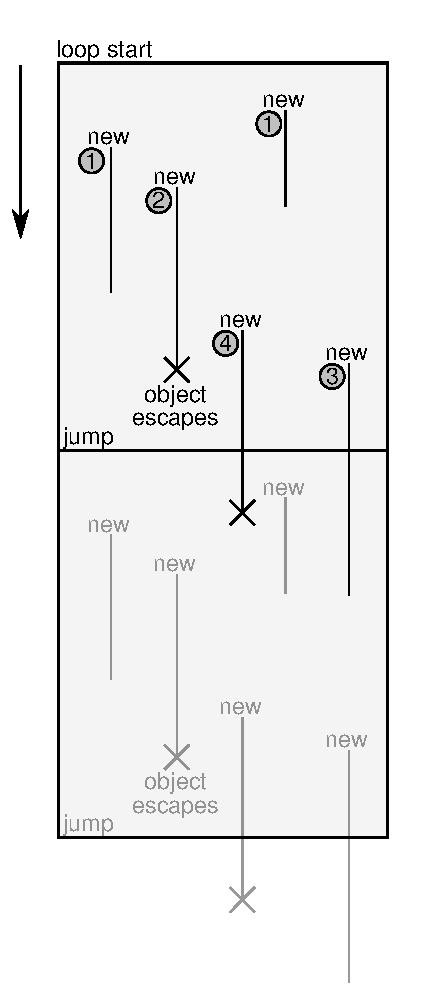
\includegraphics[scale=0.7]{figures/obj-lifetime.pdf}

\caption{Object Lifetimes in a Trace}
\label{fig:lifetimes}
\end{figure}

Figure~\ref{fig:lifetimes} shows a trace before optimization, together with the
lifetime of various kinds of objects created in the trace. It is executed from
top to bottom. At the bottom, a jump is used to execute the same loop another
time (for clarity, the figure shows two iterations of the loop). The loop is
executed until one of the guards in the trace fails, and the execution is
aborted and interpretation resumes.

Some of the operations within this trace are \texttt{new} operations, which each
create a new instance of some class. These instances are used for a while, e.g.
by calling methods on them (which are inlined into the trace), reading and
writing their fields. Some of these instances \emph{escape}, which means that
they are stored in some globally accessible place or are passed into a
non-inlined function via a residual call.

Together with the \texttt{new} operations, the figure shows the lifetimes of the
created objects. The objects that are created within a trace using \texttt{new}
fall into one of several categories:

\begin{itemize}
    \item Category 1: Objects that live for a while, and are then just not
    used any more.

    \item Category 2: Objects that live for a while and then escape.

    \item Category 3: Objects that live for a while, survive across the jump to
    the beginning of the loop, and are then not used any more.

    \item Category 4: Objects that live for a while, survive across the jump,
    and then escape. To these we also count the objects that live across several
    jumps and then either escape or stop being used.\footnote{In theory, the
    approach of Section~\ref{sec:XXX} works also for objects that live for
    exactly $n>1$ iterations and then don't escape, but we expect this to be a
    very rare case, so we do not handle it.}
\end{itemize}

The objects that are allocated in the example trace in
Figure~\ref{fig:unopt-trace} fall into categories 1 and 3. Objects stored in
\texttt{p5, p6, p11 XXX} are in category 1, objects in \texttt{p10, p15} are in
category 3.

The creation of objects in category 1 is removed by the optimization described
in Section~\ref{sec:virtuals}. XXX

\section{Escape Analysis in a Tracing JIT}
\label{sec:virtuals}


\subsection{Virtual Objects}

The main insight to improve the code shown in the last section is that objects
in category 1 don't survive very long -- they are used only inside the loop and
nobody else in the program stores a reference to them. The idea for improving
the code is thus to analyze which objects fall in category 1 and may thus
not be allocated at all.

XXX is "symbolic execution" the right word to drop?

This process is called \emph{escape analysis}. The escape analysis of
our tracing JIT works by using \emph{virtual objects}: The trace is walked from
beginning to end and whenever a \texttt{new} operation is seen, the operation is
removed and a virtual object\footnote{XXX what I have in mind when I talk
of ``virtual object'' is the run-time behavior -- i.e. a real object that
would exist at run-time, except that it has be virtual-ized.  Here you seem
to mean rather ``virtual object description'' or something.}
is constructed. The virtual object summarizes the
shape of the object that is allocated at this position in the original trace,
and is used by the optimization to improve the trace. The shapes describe
where the values that would be stored in the fields of the allocated objects
come from. Whenever the optimizer sees a \texttt{setfield} that writes into a virtual
object, that shape summary is thus updated and the operation can be removed.
When the optimizer encounters a \texttt{getfield} from a virtual, the result is read
from the virtual object, and the operation is also removed.

XXX what happens on a guard\_class?

In the example from last section, the following operations would produce two
virtual objects, and be completely removed from the optimized trace:

\begin{verbatim}
p5 = new(BoxedInteger)
setfield_gc(p5, i4, intval)
p6 = new(BoxedInteger)
setfield_gc(p6, -100, intval)
\end{verbatim}


The virtual object stored in \texttt{p5} would know that it is an \texttt{BoxedInteger}, and that
the \texttt{intval} field contains \texttt{i4}, the one stored in \texttt{p6} would know that
its \texttt{intval} field contains the constant -100.

The following operations, that use \texttt{p5} and \texttt{p6} could then be
optimized using that knowledge:

\begin{verbatim}
guard_class(p5, BoxedInteger)
i7 = getfield_gc(p5, intval)
# inside BoxedInteger.add
guard_class(p6, BoxedInteger)
# inside BoxedInteger.add__int
i8 = getfield_gc(p6, intval)
i9 = int_add(i7, i8)
\end{verbatim}

The \texttt{guard\_class} operations can be removed, because the classes of \texttt{p5} and
\texttt{p6} are known to be \texttt{BoxedInteger}. The \texttt{getfield\_gc} operations can be removed
and \texttt{i7} and \texttt{i8} are just replaced by \texttt{i4} and -100. Thus the only
remaining operation in the optimized trace would be:

\begin{verbatim}
i9 = int_add(i4, -100)
\end{verbatim}
    
The rest of the trace is optimized similarly.

So far we have only described what happens when virtual objects are used in
operations that read and write their fields. When the virtual object is used in
any other operation, it cannot stay virtual. For example, when a virtual object
is stored in a globally accessible place, the object needs to actually be
allocated, as it will live longer than one iteration of the loop.

XXX ``the trace above'' is dangerous; should mention all figures by numbers

This is what happens at the end of the trace above, when the \texttt{jump} operation
is hit. The arguments of the jump are at this point virtual objects. Before the
jump is emitted, they are \emph{forced}. This means that the optimizers produces code
that allocates a new object of the right type and sets its fields to the field
values that the virtual object has. This means that instead of the jump, the
following operations are emitted:

XXX should the variables be written in $math-style$ everywhere?

\texttt{
\begin{tabular}{l} 
$p_{15}$ = new(BoxedInteger) \\
setfield\_gc($p_{15}$, $i_{14}$, intval) \\
$p_{10}$ = new(BoxedInteger) \\
setfield\_gc($p_{10}$, $i_{9}$, intval) \\
jump($p_{15}$, $p_{10}$) \\
\end{tabular}
}

Note how the operations for creating these two instances have been moved down the
trace. It looks like for these operations we actually didn't win much, because
the objects are still allocated at the end. However, the optimization was still
worthwhile even in this case, because some operations that have been performed
on the forced virtual objects have been removed (some \texttt{getfield\_gc} operations
and \texttt{guard\_class} operations).

\begin{figure}
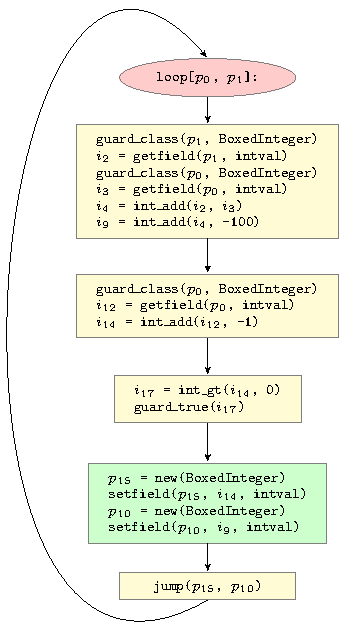
\includegraphics{figures/step1.pdf}
\label{fig:step1}
\caption{Resulting Trace After Allocation Removal}
\end{figure}

The final optimized trace of the example can be seen in
Figure~\ref{fig:step1}.

The optimized trace contains only two allocations, instead of the original five,
and only three \texttt{guard\_class} operations, from the original seven.

\subsection{Algorithm}
\label{sub:Algorithm}

XXX want some sort of pseudo-code

% subsection Algorithm (end)

%___________________________________________________________________________

\subsection{Summary}

In this section we described how simple escape analysis within the scope of one
loop works. This optimizations reduces the allocation of many intermediate data
structures that become garbage quickly in an interpreter. It also removes a lot
of the type dispatching overhead. In the next section, we will explain how this
optimization can be improved further.

XXX Category 2 The optimization of
Section~\ref{sec:virtuals} deals with them too: the \texttt{new} that creates them and
the field accesses are deferred, until the point where the object escapes.

% section Escape Analysis in a Tracing JIT (end)

\section{Escape Analysis Across Loop Boundaries}
\label{sec:crossloop}

In the last section we described how escape analysis can be used to remove
many of the allocations of short-lived objects and many of the type dispatches
that are present in a non-optimized trace. In this section we will improve the
optimization to also handle more cases.

The optimization of the last section considered the passing of an object along a
jump to be equivalent to escaping. It was thus treating objects in category 3
and 4 like those in category 2.

The improved optimization described in this section will make it possible to deal
better with objects in category 3 and 4. This will have two consequences: on
the one hand, more allocations are removed from the trace (which is clearly
good). As a side-effect of this, the traces will also be type-specialized.


%___________________________________________________________________________

\subsection{Optimizing Across the Jump}

\footnote{This section is a bit
science-fictiony. The algorithm that PyPy currently uses is significantly more
complex and much harder than the one that is described here. The resulting
behaviour is very similar, however, so we will use the simpler version (and we
might switch to that at some point in the actual implementation).}

Let's look at the final trace obtained in the last section for the example loop.
The final trace was much better than the original one, because many allocations
were removed from it. However, it also still contained allocations:

The two new \texttt{BoxedIntegers} stored in \texttt{p15} and \texttt{p10} are passed into
the next iteration of the loop. The next iteration will check that they are
indeed \texttt{BoxedIntegers}, read their \texttt{intval} fields and then not use them
any more. Thus those instances are in category 3.

In its current state the loop
allocates two \texttt{BoxedIntegers} at the end of every iteration, that then die
very quickly in the next iteration. In addition, the type checks at the start
of the loop are superfluous, at least after the first iteration.

The reason why we cannot optimize the remaining allocations away is because
their lifetime crosses the jump. To improve the situation, a little trick is
needed. The trace above represents a loop, i.e. the jump at the end jumps to
the beginning. Where in the loop the jump occurs is arbitrary, since the loop
can only be left via failing guards anyway. Therefore it does not change the
semantics of the loop to put the jump at another point into the trace and we
can move the \texttt{jump} operation just above the allocation of the objects that
appear in the current \texttt{jump}. This needs some care, because the arguments to
\texttt{jump} are all currently live variables, thus they need to be adapted.

If we do that for our example trace above, the trace looks like this:
\begin{figure}
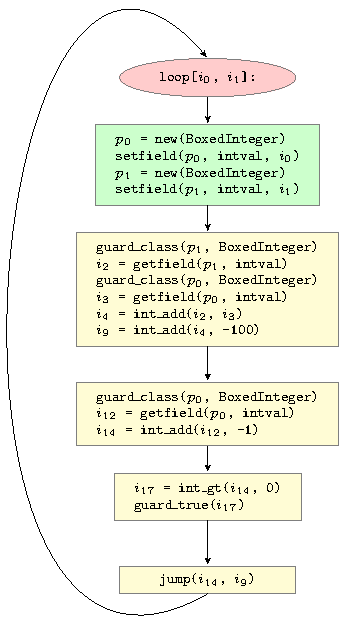
\includegraphics{figures/step2.pdf}
\end{figure}

XXX the figure is moved elsewhere by latex

Now the lifetime of the remaining allocations no longer crosses the jump, and
we can run our escape analysis a second time, to get the following trace:
\begin{figure}
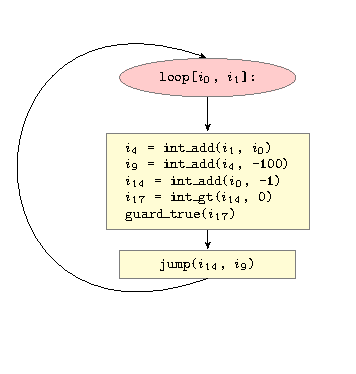
\includegraphics{figures/step3.pdf}
\end{figure}

XXX the figure is moved elsewhere by latex

This result is now really good. The code performs the same operations than
the original code, but using direct CPU arithmetic and no boxing, as opposed to
the original version which used dynamic dispatching and boxing.

Looking at the final trace it is also completely clear that specialization has
happened. The trace corresponds to the situation in which the trace was
originally recorded, which happened to be a loop where \texttt{BoxedIntegers} were
used. The now resulting loop does not refer to the \texttt{BoxedInteger} class at
all any more, but it still has the same behaviour. If the original loop had
used \texttt{BoxedFloats}, the final loop would use \texttt{float\_*} operations
everywhere instead (or even be very different, if the object model had
more different classes).


%___________________________________________________________________________

\subsection{Entering the Loop}

The approach of placing the \texttt{jump} at some other point in the loop leads to
one additional complication that we glossed over so far. The beginning of the
original loop corresponds to a point in the original program, namely the
\texttt{while} loop in the function \texttt{f} from the last section.

Now recall that in a VM that uses a tracing JIT, all programs start by being
interpreted. This means that when \texttt{f} is executed by the interpreter, it is
easy to go from the interpreter to the first version of the compiled loop.
After the \texttt{jump} is moved and the escape analysis optimization is applied a
second time, this is no longer easily possible.  In particular, the new loop
expects two integers as input arguments, while the old one expected two
instances.

To make it possible to enter the loop directly from the intepreter, there
needs to be some additional code that enters the loop by taking as input
arguments what is available to the interpreter, i.e. two instances. This
additional code corresponds to one iteration of the loop, which is thus
peeled off \cite{XXX}:

\begin{figure}
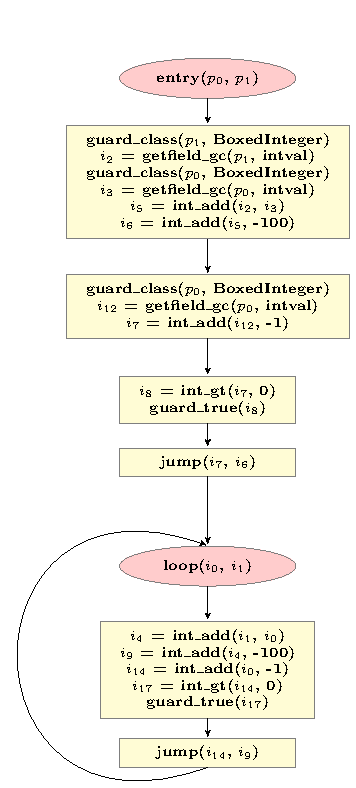
\includegraphics{figures/step4.pdf}
\end{figure}

XXX the figure is moved elsewhere by latex

XXX optimization particularly effective for chains of operations

%___________________________________________________________________________

\subsection{Summary}

The optimization described in this section can be used to optimize away
allocations in category 3 and improve allocations in category 4, by deferring
them until they are no longer avoidable. A side-effect of these optimizations
is also that the optimized loops are specialized for the types of the variables
that are used inside them.

% section Escape Analysis Across Loop Boundaries (end)

\section{Evaluation}
\label{sec:Evaluation}


\section{Related Work}
\label{sec:related}

\section{Conclusions}
\label{sec:conclusions}

\bibliographystyle{abbrv}
\bibliography{paper}

\end{document}
